\documentclass[12pt]{article}
\usepackage[left=2cm,  right=2cm,  top=2cm]{geometry}
\title{Smart_Sanskrit\_Annotator\_App}
\usepackage{hyperref}
\usepackage{graphicx}
\graphicspath{ {./images/} }
\usepackage{blindtext}
\par{\centering
		{\Huge {\textbf}{Smart Sanskrit Annotator App }
	}\bigskip\par}

        
\\ \\
\begin{document}

\section{Introduction}
The Smart Sanskrit Annotator App is an assisted application for three levels of parsing and tagging over Sanskrit text: POS Tagging, Morphological Tagging, and Semantic Tagging. It takes a Sanskrit sentence as input across multiple formats, and provides a user-friendly interface to annotate and store data with respect to a given input sentence.
Accepted Input Formats: WX, SLP, Velthius, KH

\section{Functionality Overview}
The user gives a sentence in one of the encoded forms. The input is then sent to the Sanskrit Heritage Reader Page (SHR : \href{http://sanskrit.inria.fr/}{www.sanskrit.inria.fr)}. The website takes the sentence and displays every possible form  and split of each word in the sentence. Compound words are also identified, and all possible splits are quoted. This data is scrapped from the website and is used as the basis of the application. Any new sentence that is encountered as an input is added to the database.\\ \\

\\ \\ \\ 
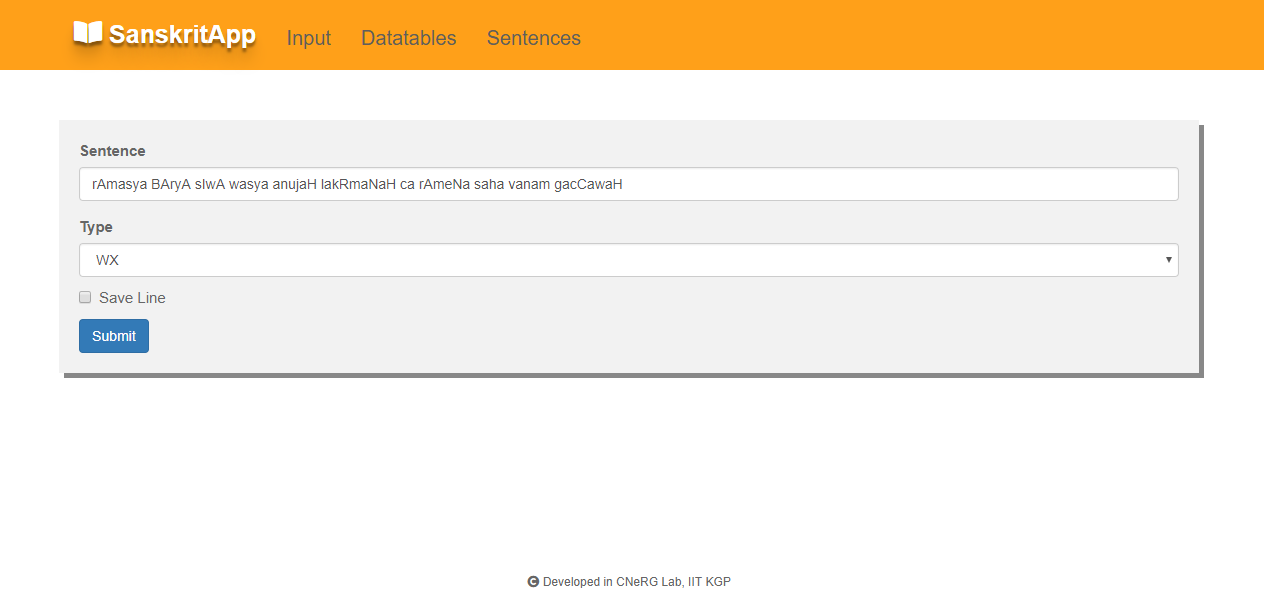
\includegraphics[width=150mm,scale=20]{capture3}\\ \\
\\ 
Segmentation option highlights the correct answers from the database.
\\ \\ 

\\ \\The grey button splitting is a unique feature that has been added for words that are not known to the annotator app, there by allowing user to edit and make changes in the button. The selected part of this button has the same functionality as that of other buttons.\\

\\The user is allowed to edit (if needed) and select one of these forms as the correct one with respect to the sentence. All other conflicting words (based on the location of the word and the possibility of sandhi) are removed automatically. Once the user is done with the POS tagging, he moves onto the Morphological and Semantic taggings.\\ \\

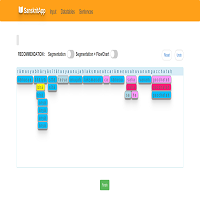
\includegraphics[width=150mm,scale=20]{capture2}\\ \\

\\The selected words appear as nodes in a flow chart with all possible morphs. The user selects the correct morph, and adds named links defining the relationship between words in the sentence. At this point in time, the user can save and download the data in tabular form as shown below. 

\section{Implementation}
The Python Django framework is used as the backend,with Jquery, Javascript, CSS and HTML to create the user interface. 
\subsection{Requirements}
\textbf{Backend- Django and Python Packages:}
\begin{itemize}
	\item python 3.6
	\item pandas
	\item bs4 (scrap data from SHR using beautifulsoup)
	\item requests
	\item django
	\item django\_datatable
	\item django\_datatables\_view
\end{itemize}
\textbf{Front End- Jquery Plugins:}
\begin{itemize}
	\item Jquery-selector : To deal with the grey\_button (unknown morph data)
	\item Jquery-flowchart : To generate the flowchart
\end{itemize}

\subsection{Backend}
The server side of the application has been created with Django 2.0, a python-based web application developer.

\textbf{Data Tables/Models:}
\begin{itemize}
	\item Sentences : Set of all sentences stored in the database
	\item Wordsinsentence : Set of users' selection
	\item Wordoptions : Stores contents of all words post scrapping from SHR
	\item annotatorapp\_indeclinables : Set of all indeclinables
	\item annotatorapp\_nouns : Set of all nouns
	\item annotatorapp\_verbs : Set of all verbs
	\item annotatorapp\_linetypes : Map each input with its encoding type
	\item annotatorapp\_user : To store user activity 
\end{itemize}

\textbf{Important View Functions:}
\begin{itemize}
	\item  getdragdata : Retrieves the saved word data (presented as draggableOperators) from the database
	\item  savedragdata : Saves current word data to the database
	\item  presentdataview : 1) Check if Input is present in the existing database (and if not) 2) Send request to SHR to scrap the data. Returns a dictionary and a pandas dataframe with the data.
	\item  savedata\_to\_db : saves flowchart data (correct morphological form and relationships) to the databse
	\item  getformdata : used to retrieve autocomplete noun/verbs/indeclinables options
\end{itemize}

The sentence is taken as an input from the user in one of the encoded formats among WX, SLP, Velthius, KH. It is sent to the Sanskrit Heritage Reader site and the results are scrapped along with word metadata such as its positioning, color\_class (each indicating a different type of word), lemma, morph, root word, etc (refer to codeforline.py getdatafromsite function). These details are stored under the Wordoptions table. A pandas dataframe "context" with all the above stated parameters is generated, along with a dictionary (conflictslp) consisting of word conflicts based on position. The corner cases for sandhi(with added check for overlapping of words) are handled and taken care of (codeforline.py contestforwordsdata()) and sent back to the client.

The user's activity- i.e, entry and exit time stamps(all the actions that are performed during this interval), the click sequence, and selected word data is stored in annotatorapp\_user. This post call is triggered as the FINISH button is clicked post completion of POS tagging by the user. Next, on completion of the rest of the tagging procedures, pressing the save data button saves the selected data in their corresponding data tables- wordoptions, linetypes, sentences, and Wordsinsentence. \\ 

Annotator\_nouns, verbs, and indeclinables contain all the possible morhps the corresponding type can take (eg nom. sg. m for noun indicates nominal, singular, masculine form). These are fetched (if) when the user wants to edit the details of a given word for a suggestion box.  \\

The final result is saved in a CoNNLu format and can be downloaded by the user.\\
\\ \textbf{Custom Commands:}\\
\\ Two custom commands are present: scrap, scrap2, scrap3 and recommendation. \\ \\Scrap is a one-time command which must be run during the initial setup of the server. The command populates the noun,verb and indeclinables tables using data from data.txt present in the same directory. These are retrieved when a user wishes to edit a given word and the different morphs of each form are displayed as options for the user to select.\\ \\ Scrap2 is another command used for running during initial setup of server and is used for loading all the example sentences along with their solutions.\\ \\ Scrap3 is also a one-time command which must be run during initial setup of the server. This command loads the sample 200 sentences from answers.txt onto a table in the db so that batches of it can be taken for testing\\ \\The recommendation command is used for purposes during the trial run of the program. It contains a set of 204 sentences along with the predictions from the ML model for the correct sentence. This command is for special cases only.

\subsection{FrontEnd}
The front end is written in Javascript, Jquery and HTML as four files:
\begin{itemize}
	\item index.html : The page which takes user input in and its encoding
	\item basic.html : Basic static template over all pages- contains defenition of nav bar and headers
	\item presentdata.html : The main annotatorapp page with the jquery functionality included
	\item tables.html : Display of stored tables
	\item exsent.html : Display of example sentences that user can give as inputs.

\end{itemize}



\subsection{Instructions to Setup the App}
1. Install required above-mentioned Django packages. (Django verson 2.0, Python version 3.x \\ 
2. python manage.py makemigrations \\ 
3. python manage.py migrate \\
4. python manage.py scrap \\
5. python manage.py scrap2 \\
6. python manage.py scrap3 \\
7. python manage.py runserver

\subsection{Flowchart - Structure}
The sequence of morphological segments that we click over and then click on finish, gets added to the database. These form the operators and the user adds links between them according to his own perusal. 

Various options that are available to this include options to save this data in tabular form, delete selected operator link, save flowchart data, get saved data downloaded, show data, hide data, edit link properties. 
\\ \\ \\
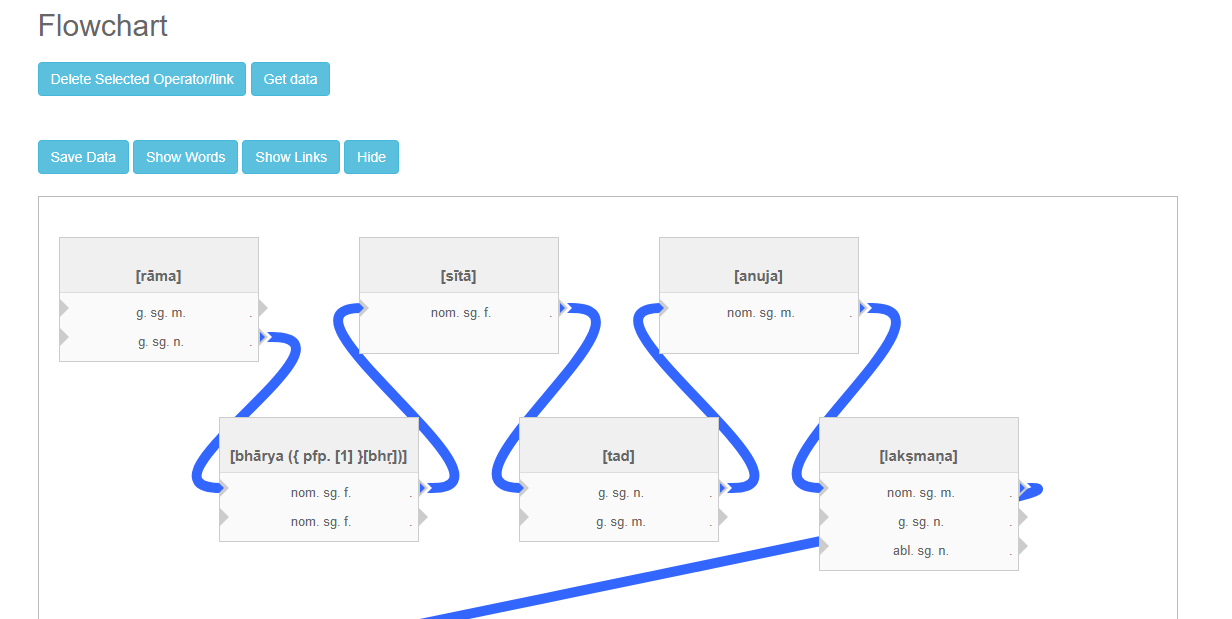
\includegraphics[width=150mm,scale=20]{capture1}
\\ \\ \\
The following is a screen shot to the editing properties of the links in the app.\\ \\ 

\\ \\ \\
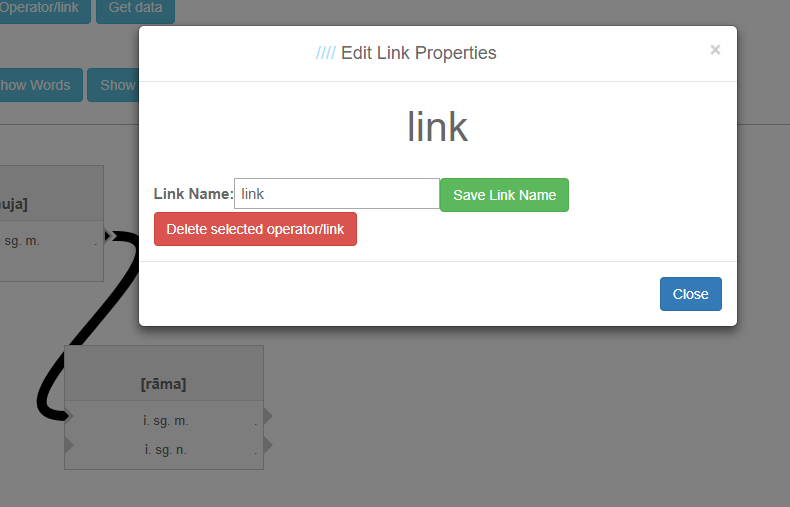
\includegraphics[width=150mm,scale=20]{capture4}
\end{document}